\chapter{Fundamentação Teórica}
\label{chap:fundteor}

\begin{flushright}

   \begin{list}{}{
      \setlength{\leftmargin}{4.5cm}
      \setlength{\rightmargin}{0cm}
      \setlength{\labelwidth}{0pt}
      \setlength{\labelsep}{\leftmargin}}
      \item Quanto maior for a rapidez de transformação de uma
      sociedade, mais temporárias são as necessidades
      individuais. Essas flutuaçõess tornam ainda mais acelerado
      o senso de turbilh da sociedade.

      \begin{list}{}{
      \setlength{\leftmargin}{0cm}
      \setlength{\rightmargin}{0cm}
      \setlength{\labelwidth}{0pt}
      \setlength{\labelsep}{\leftmargin}}
      \item (Alvin Toffler)
      \end{list}
   \end{list}
\end{flushright}

\begin{flushright}
  Quanto maior for a rapidez de transformação de uma \\
  sociedade, mais temporárias são as necessidades \\
  individuais. Essas flutuações tornam ainda mais \\
  acelerado o senso de turbilhão da sociedade. \\
  \ \\
  (Alvin Toffler)
\end{flushright}

%--------- NEW SECTION ----------------------
\section{Ultra Wide Band}
\label{sec:sota}
O princípio de funcionamento do Pozyx se dá na utilização da tecnologia 
de Ultra Wide Band (UWB) ou de banda ultra larga. UWB é um protocolo de comunicação sem fio
assim como o Wi-fi e o Bluetooth. Contudo, seu funcionamento difere um pouco destas e outras tecnologias,
trazendo vantagens e desvantagens. O uso e os estudos acerca da tecnologia UWB vêm se desenvolvendo
há cerca de 100 anos, quando o inventor e físico italiano Guglielmo Marconi (1874-1937), baseando-se na teoria 
de Maxwell sobre ondas eletromagnéticas, estudava os princípios da transmissão de dados por radiofrequência. Futuramente 
foi utilizada em radares do exército estado-unidense e, entre os anos de 1960 a 1990 ficou restrita aplicações militares.

%--------- NEW SECTION ----------------------
\section{Características da tecnologia}
\label{sec:ass1}
Como mencionado anteriormente, a tecnologia UWB possui algumas diferenças de funcionamento,
quando comparada a outras de comunicação \textit{Wireless}. 

\subsection{Vantagens}
Sua principal vantagem é a larga banda de frequência na qual pode operar: aproximadamente 500 MHz, 
enquanto as do Wi-fi e Bluetooth são de algumas dezenas de MHz. Essa grande largura de banda torna 
os sinais menos susceptíveis a interferências, oriunda de ondas emitidas por outros aparelhos ao redor.
A Figura 2.1 ilustra essa diferença.

\begin{figure} [h!]												 
	\centering													 
	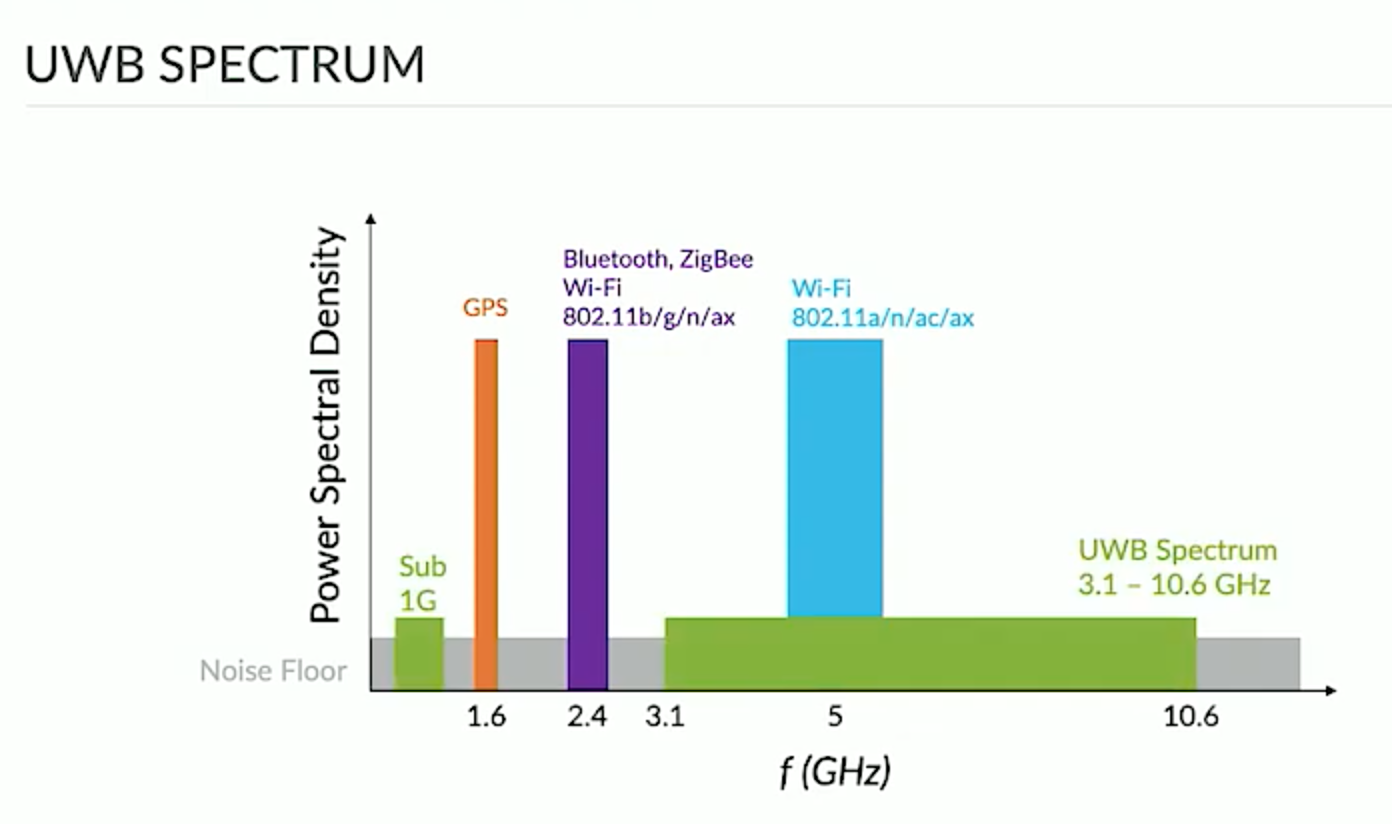
\includegraphics[width=0.8\textwidth]{./uwb_spectrum}				 
	\caption{Insufficient data.}		
	\label{img:ihuma}												 
\end{figure}

Outra característica do UBW é a utilização de rápidos pulsos (em média 2 ns entre as bordas de subida e descida) para transmitir dados, 
que são muito mais eficientes e precisos do que por alteração da frequência ou amplitude do sinal. Essa é uma das características
que fazem desta tecnologia muito útil para localização \textit{indoor}, podendo apresentar uma precisão de menos de 15 cm,
quanto outras tecnologias não chegam a 1 metro.

Uma das grandes dificuldades em localização \textit{indoor} é a perda do sinal ao ser refletido em paredes ou outros obstáculos. Considerando sinais
senoidais, a interferência entre o sinal emitido e refletido pode alterar o sinal a ponto de sua frequência e amplitude não serem
mais reconhecidas pelo receptor. Por utilizar pulsos e trabalhar numa ampla faixa de frequência, os sinais do UWB se mostram mais 
eficientes nessas situações, visto que são menos susceptíveis a estas alterações. 

Como pode ser visto na imagem acima, o UWB trabalha em uma potência significativamente mais baixa do que as outras tecnologias em 
toda sua banda, o que deixa aparelhos alimentados por baterias, como robôs móveis, muito mais eficientes, visto que gastariam menos energia
para se localizar.

\subsection{Desvantagens}
Em contrapartida às características supracitadas, UWB ainda têm sua aplicabilidade restrita por alguns fatores.
Por ser uma tecnologia ainda não muito explorada no mercado, seus equipamentos de instalação ainda são caros. Além disso,
o alcance máximo de um sinal em UWB é de, em média, 10 metros, tornando necessário o posicionamento de vários \textit{anchors} para que
o posicionamento em locais grandes se torne eficiente, o que encarece ainda mais o sistema.

\section{Aplicações na robótica}
A tecnologia Pozyx se assemelha com as RFID e BLE, pois para a localização de um objeto utiliza-se a estratégia de introduzir um elemento que emita um sinal e outro que capta este sinal. Estes elementos são as tags e as âncoras (anchors), o primeiro elemento se encontra no objeto e as âncoras são referências que possuem localização conhecida pelo servidor no ambiente. 

Nesta implementação, uma estratégia sugerida é chamada de variação bidirecional (TWR), na qual a tag envia um conjunto de sinais que irá atingir as âncoras ao redor e retornar,  de modo que a distância é calculada com base no tempo de viagem do sinal (TOF), uma vez que a velocidade de uma onda de rádio é conhecida. Vale ressaltar, que este processo é validado somente quando a tag consegue atingir três ou mais âncoras, pois assim o objeto irá se encontrar entre a melhor interseção dos raios dos elementos de referência, este procedimento é chamado de triangulação. Entretanto, quando há mais tags no ambiente, um elemento é tomado como referência para os demais, master tag, pois irá receber a localização das demais e se conectar a um servidor. Outra estratégia oferecida pelo fabricante é a Diferença de horário de chegada (TDOA), na qual as tags irão apenas irão apenas transmitir periodicamente um pulso UWB, e não mais esperar um retorno. Este sinal incluirá um ID da tag e será captado por todas as âncoras no alcance, as quais irão transmitir ao servidor, por meio de linhas de Ethernet, o momento exato que cada uma identificou a tag, sendo assim, com base na diferença destes horários  é possível estimar a posição da tag por meio da interseção das hipérboles definidas pelas diferenças de tempos. Nesta operação é imprescindível que a assim como a localização das âncoras sejam conhecidas, os relógios entre elas devem estar sincronizados com muita precisão. A TDOA é uma ótima opção ao considerar situações com altas taxas de atualização de informações. 

De modo geral, a tecnologia possui um grau de precisão bom, porém assim como todo método de localização, ainda se possui erros. Desse modo, em estudos recentes foi possível diminuí-los utilizando algoritmos para a diminuição de erro como o EFK, Extended Kalman Filter, [1], o qual calcula uma aproximação linear para um conjunto de funções não lineares com base na expansão de Taylor de primeira ordem.

Além da localização de robôs em ambientes indoors, o Pozyx tem estado também em aplicações de logísticas nos setores industriais, como em um estudo de caso [2] em que uma determinada empresa possuía uma má administração do  armazenamento de produtos diversos e em pequenos lotes. Neste caso, com a implementação de um sistema de identificação de paletes, utilizando tal tecnologia, foi possível mapear o armazém, sendo assim, a operação reduziu a quantidade de erros, graças a precisão da localização das mercadorias, o que ocasionou um aumento de eficiência no armazém em 3%.

Além dessa aplicação, a tecnologia foi também comprovada em uma situação de extrema movimentação, como nos esportes, quando foi utilizada para a localização de jogadores em [3]. Neste estudo foram implementados também algoritmos de filtragem, filtro de kalman e filtro de partículas, o qual resultou em um erro de localização de 31%, com erros médios de 20 cm. 




%---------------picture------------------------------------
% \begin{figure}
%     \centering
%     \subfigure[Figure A]{\label{fig:a}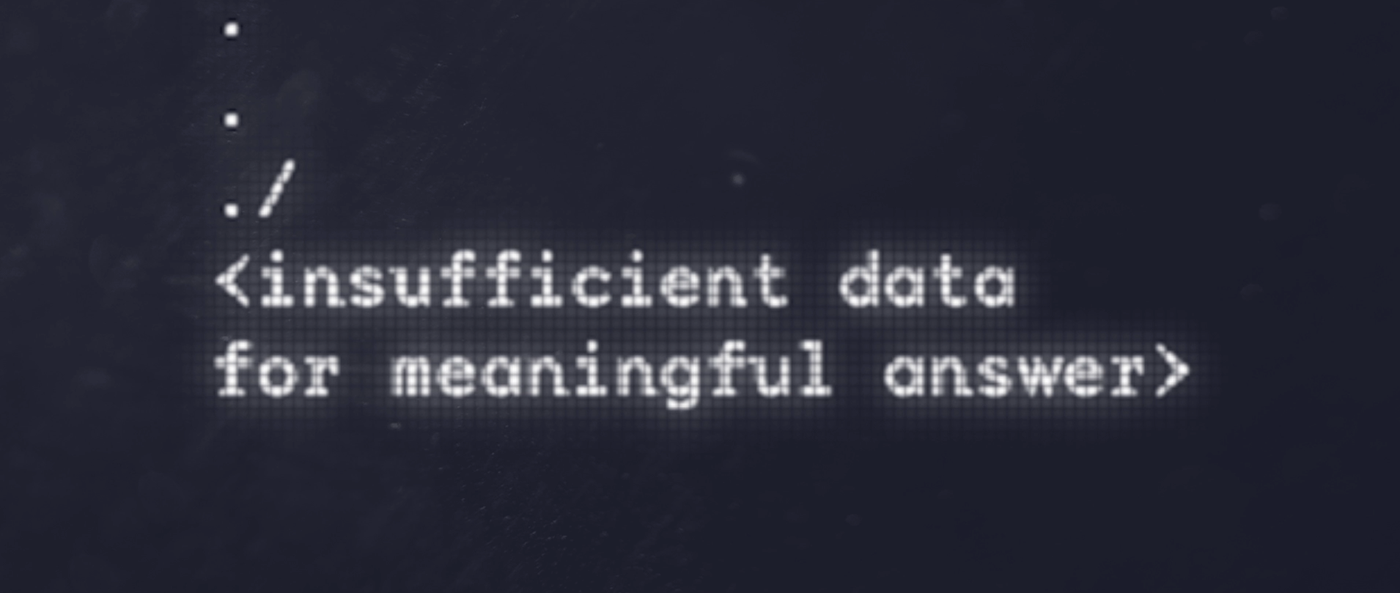
\includegraphics[width=60mm]{./lq}}
%     \subfigure[Figure B]{\label{fig:b}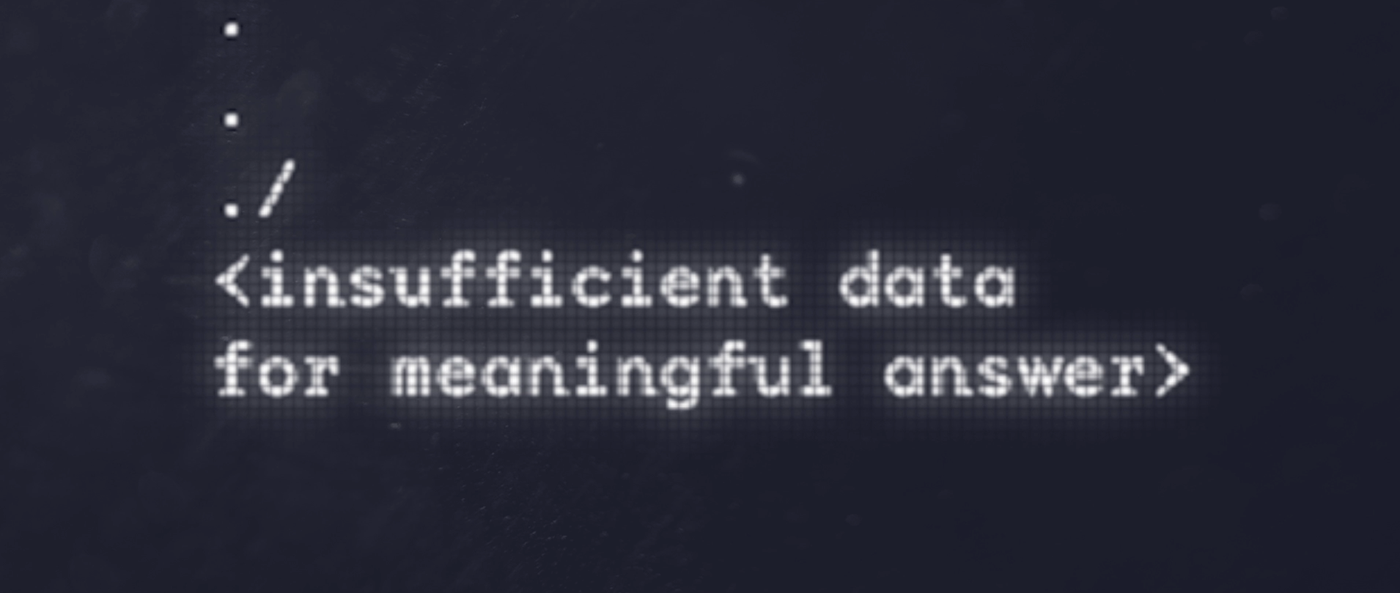
\includegraphics[width=60mm]{./lq}}
%     \subfigure[Figure C]{\label{fig:c}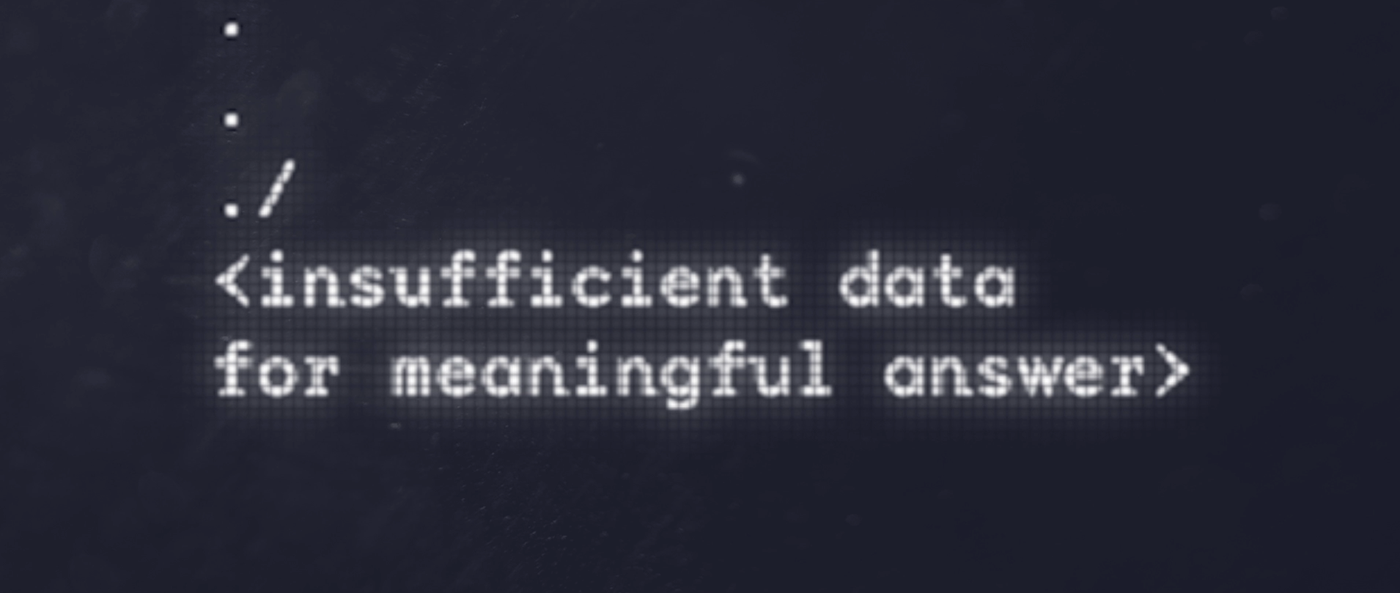
\includegraphics[width=\textwidth]{./lq}}
%     \caption{Three simple graphs}
%     \label{fig:three graphs}
% \end{figure}
%----------------------------------------------------------